\section{Theorie}
\label{sec:Theorie}


Im Folgenden wird der Operationsverstärker als zentrales Bauteil der verschiedenen Messreihen vorgestellt.
Darüberhinaus werden die damit verbundenen Schaltungen und deren verschiedene Funktionen dargestellt.
Im Übrigen wird der Unterschied zwischen idealem und realem Operationsverstärker näher beleuchtet.

\subsection{Der Operationsverstärker}

Ein Operationsverstärker ist ein spannungsgesteuerter Spannungsverstärker.
In Abbildung \ref{fig:OP}

\begin{figure}
    \centering 
    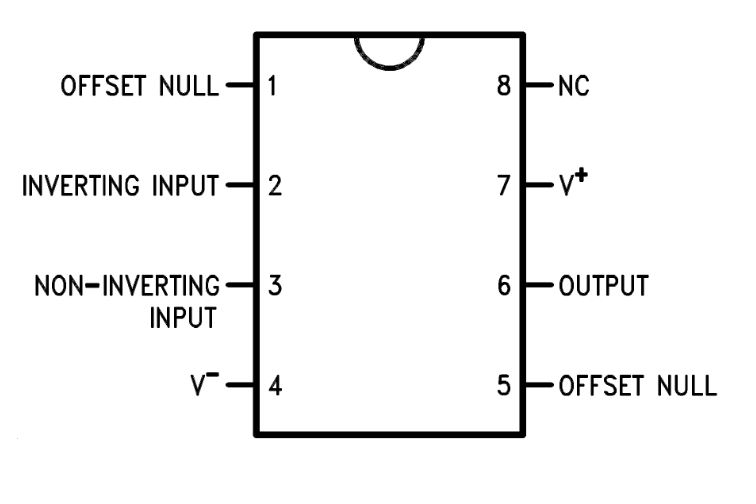
\includegraphics[width=.5\textwidth]{Bilder/OP.PNG}
    \caption{Anschlüsse eines LM741 Operationsverstärkers (\cite{LM741}).}
    \label{fig:OP}
\end{figure}

sind die Anschlüsse eines Operationsverstärkers vom Typ LM741 dargestellt.
Es gibt einen \textit{invertierenden} und einen \textit{nichtinvertierenden} Eingang.
Außerdem wird an die Anschlüsse $V^+$ und $V^-$ eine Versorgungsspannung gelegt.
Diese unterscheidet sich nur im Vorzeichen; ist also betragsmäßig gleich.
Am \textit{Output} befindet sich der Anschluss für die Ausgangsspannung.



Allgemein sorgt ein Operationsverstärker für eine Erhöhung der Eingangsspannung, wobei Ein- und Ausgangsspannung üblich in dem Zusammenhang
\begin{equation}
    U_A = v_0U_E 
\end{equation}
stehen.
$v_0$ gibt dabei die Leerlaufverstärkung an.
Dies gilt aber nur in dem nicht übersteuerten Bereich.
Der Bereich der Leerlaufverstärkung wird über die Höhe der Versorgungsspannung festgelegt.
Jenseits dieses Intervalls bleibt die Verstärkung konstant.
In Abbildung \ref{fig:Kennlinie} ist eine typische Kennlinie dargestellt.
Die Verstärkung beläuft sich auf Größenordungen von $v \propto 10^4$.


\begin{figure}
    \centering 
    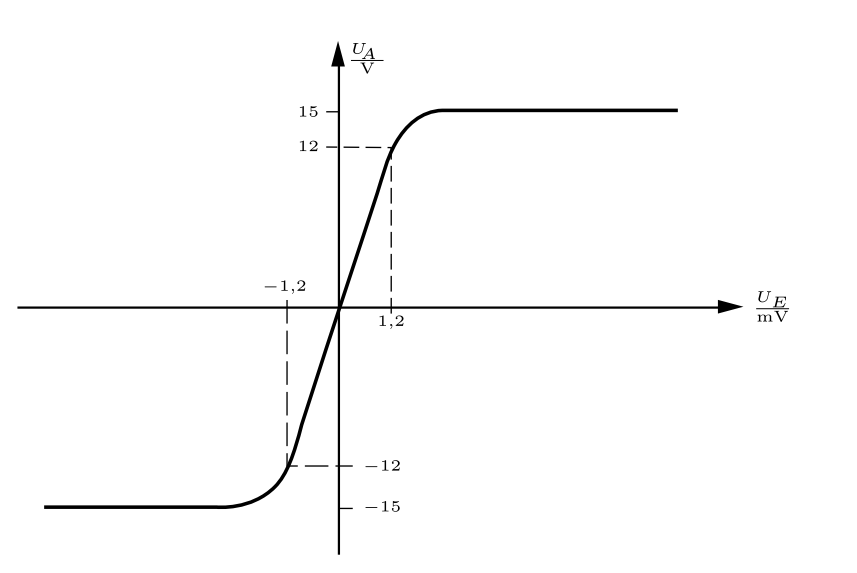
\includegraphics[width=.8\textwidth]{Bilder/Kennlinie.PNG}
    \caption{Beispiel für eine Kennlinie eines Operationsverstärkers (\cite[S.~99]{Clausert}).}
    \label{fig:Kennlinie}
\end{figure}





\begin{figure}
    \centering 
    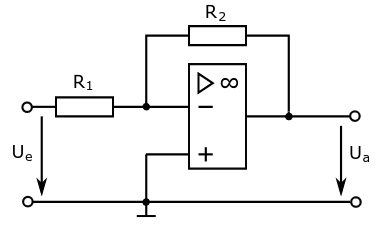
\includegraphics[width=.5\textwidth]{Bilder/Inv_Lin.png}
    \caption{Schaltbild eines invertierenden Integrators.}
    \label{fig:Inv_Lin}
\end{figure}



\begin{figure}
    \centering 
    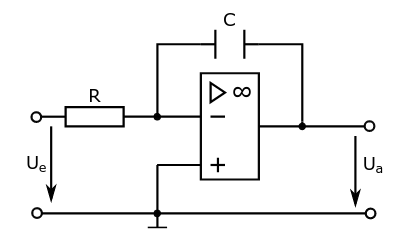
\includegraphics[width=.5\textwidth]{Bilder/Um_Int.png}
    \caption{Schaltbild eines Umker-Integrators.}
    \label{fig:Um_Int}
\end{figure}

\begin{figure}
    \centering 
    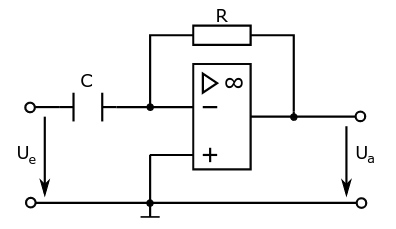
\includegraphics[width=.5\textwidth]{Bilder/Inv_Dif.png}
    \caption{Schaltbild eines invertierenden Differenzierers.}
    \label{fig:Inv_Dif}
\end{figure}

\begin{figure}
    \centering 
    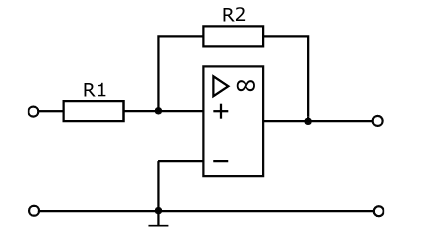
\includegraphics[width=.5\textwidth]{Bilder/Schmitt.png}
    \caption{Schaltbild eines nichtinvertierenden Schmitt-Triggers.}
    \label{fig:Schmitt}
\end{figure}

\begin{figure}
    \centering 
    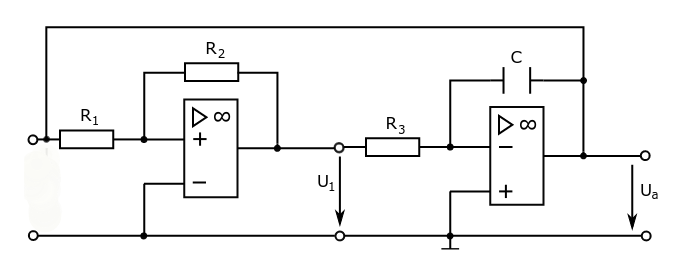
\includegraphics[width=.9\textwidth]{Bilder/Signal.png}
    \caption{Schaltbild eines Signalgenerators aus der Reihe eines nichtinvertierenden Schmitt-Triggers und eines Umker-Integrators.}
    \label{fig:Signal}
\end{figure}
%In knapper Form sind die physikalischen Grundlagen des Versuches, des Messverfahrens, sowie sämtliche für die Auswertung erforderlichen Gleichungen darzustellen. (Keine Herleitung)

%(eventuell die Aufgaben)

%Der Versuchsaufbau: Beschreibung des Versuchs und der Funktionsweise (mit Skizze/Bild/Foto)
